In this section we introduce the basic concepts of the implementation of multiplayer game development for Casanova 2. This implementation aims to relieve the programmer of the complexity of hard-coding the network implementation for an online game, while preserving encapsulation in code. We show that code analysis is required to generate the appropriate network primitives to send and receive data. Finally, we present a simple multiplayer game to show a concrete example.

\section{Introduction}
Adding multi-player support to games is a highly desirable feature. By letting players interact with each other, new forms of gameplay, cooperation, and competition emerge without requiring any additional design of game mechanics \cite{granberg2014david}. This allows a game to remain fresh and playable, even after the single player content has been exhausted. For example, consider any modern AAA (AAA refers to games with the highest development budgets\cite{wolf2008video}) game such as \textit{Halo 4}. After months since its initial release, most players have exhausted the single player, narrative-driven campaign. Nevertheless the game remains heavily in use thanks to multiplayer modes, which in effect extended the life of the game significantly. This phenomenon is even more evident in games such as \textit{World of Warcraft} or \textit{EVE}, where multiplayer is the only modality of play and there is no single-player experience.

\paragraph{Challenges}
Multi-player support in games is a very expensive piece of software to build. Multiplayer games are under strong pressure to have very good \textit{performance} \cite{claypool2006latency}. Performance is both expressed in terms of CPU time and in bandwidth used. Also, games need to be very \textit{robust} with respect to transmission delays, packets lost, or even clients disconnected. To make matters worse, players often behave erratically. It is widespread practice among players to leave a competitive game as soon as their defeat is apparent (a phenomenon so common to even have its own name: ``rage quitting'' \cite{rage_quitting}), or to try to abuse the game and its technical flaws to gain advantages or to disrupt the experience of others.

Networking code reuse is quite low across titles and projects. This comes from the fact that the requirements of every game vary significantly: from turn-based games that only need to synchronize the game world every few seconds, and where latency is not a big issue, to first-person-shooter games where prediction mechanisms are needed to ensure the smooth movement of synchronized entities, to real-time strategy games where thousands of units on the screen all need to be synchronized across game instances \cite{smed2002aspects}. In short, previous effort is substantially inaccessible for new titles. 

Encapsulation suffers from this ad-hoc nature of the implementation of the networking layer in multiplayer games. Indeed managing the information about game updates over a network requires each game entity to interface the game logic code with network connection and socket objects, data transmission method calls such as send and receive, and support data structures to manage traffic and track the status of common protocols. This happens because each game entity must provide the following functionality in order to work in a multiplayer game:

\begin{itemize}
	\item Update the logic in the fashion of a singleplayer counterpart.
	\item Choose what data is necessary to send over the network and create the message containing this information.
	\item Choose what data can be lost and what data must always be received by the other clients.
	\item Periodically check if incoming messages contain information that needs to be read and to perform specific updates.
\end{itemize}

Combining these requirements together within the same entity breaks encapsulation because now the logic of the entity and lots of spurious details only relevant to the networking implementation are mixed together, resulting in a highly noisy program. Maintenance then becomes very hard, as every change in the game logic must also be reflected in the networking implementation.

\paragraph{Existing approaches}
Networking in games is usually built with either very low-level or very high-level mechanisms. Very low-level mechanisms are based on manually sending streams of bytes and serializing only the essential bits of the game world, usually incrementally, on unreliable channels (UDP). This coding process is highly expensive because building by hand such a low-level protocol is difficult to get right, and debugging subtle protocol mismatches, transmission errors, etc. will take lots of development resources. Low-level mechanisms must also be very robust, making the task even harder.

High-level protocols such as RDP, reflection-based serialization, frameworks (such as Pastry, netty.io), etc. can also be used. These methods greatly simplify networking code, but are rarely used in complex games and scenarios. The requirements of performance mean that many high-level protocols or mechanisms are insufficient, either because they are too slow computationally (especially when they rely on reflection or events) or because they transmit too much data across the network.

\section{Motivation}

To avoid the problems of both existing approaches, we propose a middle ground. We observe that networking fundamental abstractions upon which the actual code and protocols are built do not vary substantially between games, even though the code that needs to be written to implement them does. The similarity comes from the fact that the ways to serialize, synchronize, and predict the behaviour of entities are relatively standard and described according to a limited series of general ideas. The difference, on the other hand, comes from the fact that low-level protocols need to be adapted to the specific structure of the game world and the data structures that make it up. Until now, common primitives have not been syntactically and semantically captured inside existing domain-specific languages for game development \cite{bhatti2009domain}. Using the right level of abstraction, these general patterns of networking can be captured, while leaving full customization power in the hand of the developer (to apply such primitives to any kind of game).

\section{Related work}
In the following we discuss some existing networking tools used in game development and we highlight some issues that arise from their use.

\paragraph{The Real time framework (RTF)} RTF \cite{glinka2007rtf} is a middleware built for C++ to relieve the programmer from dealing with data compression. It is more flexible than solutions based on game engines or hand-made implementations, since it automates the process of data transmission. Moreover, it supports distributed server management. Unfortunately, this solution has several flaws:
\begin{itemize}
	\item All entities must inherit from the class \texttt{Local} and the semantics of the position is pre-determined, often clashing with rendering or physics.
	\item Platform independence requires that the programmer uses RTF primitive	types.
	\item Data transmission automation requires that all game entities inherit the class \texttt{Serializable}.
	\item Being a middleware, RTF is not aware of what games are going to use it for (every game comes with different data structures). Thus, the developer is tasked to include in his code also logic to update the RTF layer, in order to keep the game updated over the network.
\end{itemize}


\paragraph{Network scripting language (NSL)} NSL \cite{russell2008tackling} provides a language extension based on a send-receive mechanism. Moreover it provides a built-in client side prediction (a feature missing in existing highly concurrent and distributed languages such as Stackless Python \cite{kalogirou2005multithreaded} and Erlang \cite{armstrong1993concurrent}), which is periodically corrected by the server. 

\paragraph{Unreal Engine/Unity Engine} Unreal Engine \cite{games2006unreal} and Unity Engine \cite{engine9unity} are commercial game engines supporting networking.  Both Unity and Unreal Engine use a client-server approach. In Unreal Engine, the server contains the ``true'' game state, and the clients contain a ``dirty'' copy, which is validated periodically. It is possible to define entities (actors in Unreal Engine jargon) that are replicated on the clients. Whenever a replicated actor changes on the server, this change is also reflected on the clients. Additional customization can be achieved through Remote procedure calls (RPCs) of three kinds.
\begin{itemize}
	\item The function is called on the server and executed on the client. This is used for game elements that do not affect gameplay, such as creating a particle effect when a weapon is fired.
	\item The function is called on the client and executed on the server. This is useful for events that affect the other clients and should be validated by the server.
	\item The function is executed in multi-cast, meaning that the server calls the function and that it is executed on both the server and all the clients.
\end{itemize}

The Unity Engine uses a similar approach based on networking components, synchronized at every frame, and RPC's to define custom synchronization events.

Unfortunately, customization comes at the cost of the level of detail that developers must face. Using RPC's require a deep knowledge of the engine and writing lots of code, as discussed in Section \ref{Common issues}.

In this section we introduce a small example that addresses the requirements of designing a multiplayer game. We then present an architecture that aims to fulfil these requirements.

\section{The master/slave network architecture}

We chose to implement the networking layer in Casanova 2 by using a peer-to-peer architecture for the following reasons:

\begin{itemize}
	\item Server-client architectures are more reliable but suitable only for specific genres of games (mostly Shooter games), while other genres, such as Real-time strategy games or Online Role Playing Games, use P2P architectures.
	\item We do not have to write a separate logic for an authoritative game server, which has to validate the actions of clients.
\end{itemize}

Casanova will provide a generic tracking server, which is run separately from the main program. The tracking server is a thin service that connects players participating in a single game, and helps with forwarding the network traffic through NATs (Network Address Translation).

Each client maintains a local copy of the \texttt{world} entity and has direct control over a single portion of it. Instances belonging to such as portion are seen as \textit{master} by this player, who is always allowed to directly change the state of the master instances without having to validate this state change by synchronizing with other players through the network.

Each client also maintains a portion of the world that is not directly under his control. Instances belonging to such as portion are seen as \textit{slave} by this player, who is only allowed to \textit{predict} the local state of the instances and, whenever he receives an update from their masters, must correct this prediction according to the data contained in the received messages. The slave part of the world is thus maintained passively by the client: the only active part is predicting the evolution of the entity state and correcting it whenever he receives an update by its master.

For this purpose, we extend the syntax of Casanova rules by allowing them to be marked with the modifiers \texttt{master} and \texttt{slave}. These rules are executed respectively on master and slave entities. Note that it is still possible not to mark a rule with these modifiers, which means that the rule is always executed independently of the fact that the entity is either master or slave on that particular client. We also allow to mark a rule as \texttt{connecting} and \texttt{connected}. These rules are triggered only once respectively when a new client connects and when the clients detect a new connection.

Casanova also provides primitives to send (reliably or unreliably) and receive data. A schematic representation of this architecture can be seen in Figure \ref{fig:masterslave}.

\begin{figure}[h!]
	\centering
	\caption{Representation of the game world in a networking scenario}
	\label{fig:network_world}
	\begin{subfigure}[t]{0.3\linewidth}
		\centering
		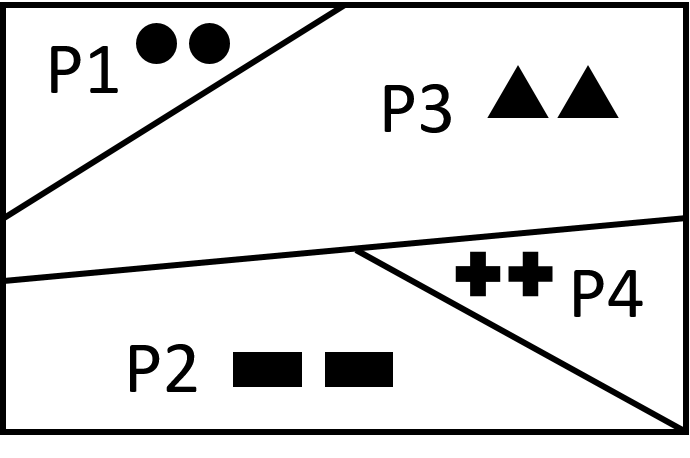
\includegraphics[width=1\linewidth]{Figures/networking2}
		\caption{Unknown correct game state when P3 joins the game.\\}
		\label{subfig:networking_ideal}
	\end{subfigure}
	\begin{subfigure}[t]{0.3\linewidth}
		\centering
		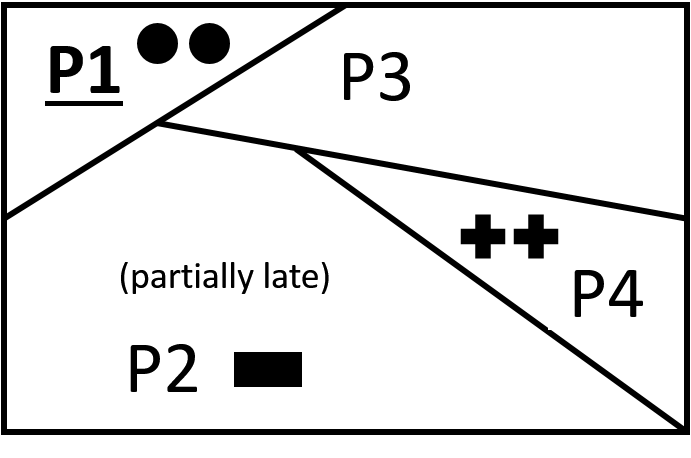
\includegraphics[width=1\linewidth]{Figures/networking1}
		\caption{Networking game state seen from the point of view of P1. P2 is partially synchronized, P4 is fully synchronized, and P3 is a new client that is late and is still sending its data}
		\label{subfig:networking_relative}
	\end{subfigure}
	
	
\end{figure}

\begin{figure}
	\centering
	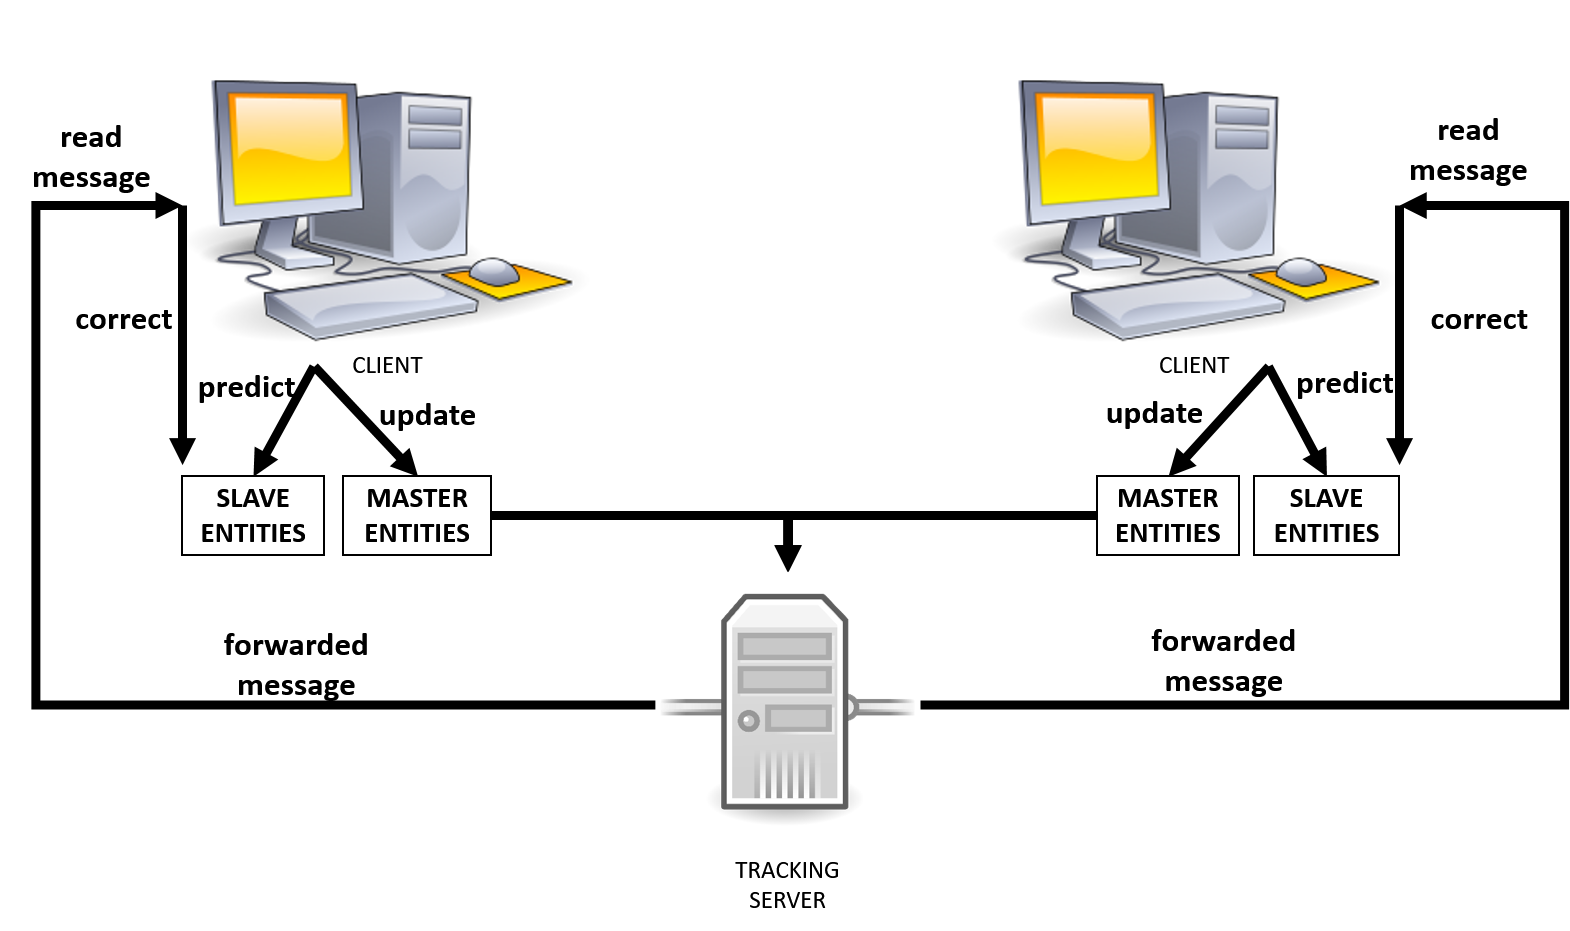
\includegraphics[width = \textwidth]{Figures/masterslave}
	\caption{master/slave architecture}
	\label{fig:masterslave}
\end{figure}

Note the aim of this architecture is to provide language-level primitives to describe the networking logic. This means that the compiler will be able to generate code compatible with the low-level network libraries that provide transmission functions over the network channel without having to change Casanova code in the program. In our implementation, we chose the .NET library \texttt{Lidgren}, which is widely used also in commercial game engines such as Unity3D and MonoGame, but nothing prevents the compiler to be expanded in order to target other similar libraries for other languages, such as jgroups \cite{ban2002jgroups}.

\section{Case study}
Let us consider a simple shooter game where each player controls a space ship. Players can move forward, backward, and rotate the ship to change direction. Moreover, they can use the ship lasers to shoot other players. If a laser hits an enemy ship, we increase the player's score. Designing such a game requires to address the following issues, depicted by the schematic representation in Figure \ref{fig:network_world}:

\begin{enumerate}
	\item Each player must maintain a local version of the game state (world). In order to avoid to flood the network with messages, all the copies are not fully synchronized at each frame, thus they are slightly different and each client knows the latest version of only part of the copy.
	\item A player \texttt{connecting} to an existing game must be able to receive the latest update of the game state and send the new ship he will control to existing players in the game.
	\item A player already \texttt{connected} to the game must detect a new connection and send his master portion of the game state.
	\item Each player must be able to control only one ship at a time. This means that the part of the game logic that processes the input and modifies the spatial data of the ship (position and rotation) should only be executed on the ship controlled by the player and not on the local copies of other players' ships. This means that each player sees as \texttt{master} only one ship instance.
	\item Each player must send the updated state of the ship he controls to the other players after executing the local update. To achieve better performance over the network, the data is not sent at every update, but with a lower frequency.
	\item Each player must receive the updated state of \texttt{slave} ships controlled by other players. In this phase, we must take into account that, as explained above, not every update is sent, so the player should ``predict'' what will happen during the game frames in which he does not receive an update.
\end{enumerate}

\section{Implementation}
Each of the scenarios described above requires specific language extensions. These extensions identify connection, ownership (master/slave), and various send and receive primitives. In this section, we introduce each primitive by using a multiplayer game example \footnote{The game source code and executable can be found at \url{https://github.com/vs-team/casanova-mk2/wiki/Networking-extension}}. We now give an implementation of the shooter game presented above, using the extended version of Casanova 2 with network primitives. 

The \texttt{world} contains a list of ships controlled by each player.
\begin{lstlisting}
world Shooter = {
Ships  : [Ship]
...
}
\end{lstlisting}

Each \texttt{Ship} contains a position, a rotation, a collection of shot projectiles, and the score.
\begin{lstlisting}
entity Ship = {
Position   : Vector2
Rotation   : float32
Projectiles : [Projectile]
Score		  : int
...
}

\end{lstlisting}

Each \texttt{Projectile} contains its position and velocity.

\begin{lstlisting}
entity Projectile = {
Position : Vector2
Velocity : Vector2
...
}
\end{lstlisting}

\subsubsection{Connection}
When a player connects, we must consider two different situations: (\textit{i}) a player is already in the game and must send the current game state to the connecting players, and (\textit{ii}) the player who is connecting needs to send the ship he will instantiate and control (its initial state). Both the players in the game and the connecting one must receive the game states that are sent. For this purpose we introduce two additional modifiers, \texttt{connecting} and \texttt{connected}, that can be added to rule declarations to mark their role in the multiplayer logic.

\paragraph{Connecting} A rule marked with \texttt{connecting} is executed once when a player joins the game for the first time. In our example, the player should send his initial state (the created ship) to the other players. We use the primitive \texttt{send\_reliable} because we must be sure that eventually all players will be notified of the ship creation.
\begin{lstlisting}
world Shooter = {
...
rule connecting Ships =
yield send_reliable Ships
}
\end{lstlisting}

\paragraph{Connected} A rule marked with \texttt{connected} is run whenever a new player joins the game by all existing players. When this occurs, each player sends its ship. The system will take care to send only the ship controlled locally by the player itself for each player. The rule will use the \texttt{send\_reliable} primitive for the same reason explained in the previous point.

\begin{lstlisting}
world Shooter = {
...
rule connected Ships =
yield send_reliable Ships
}
\end{lstlisting}

Note that even if the code is the same, the semantics of the two rules are different. The first one is executed by the player joining the game, who locally instantiates its \texttt{Ship} and must send its list of \texttt{Ships} (containing only the local instance) to the other players. The second one is executed by all existing players who must share with the joining player the list of existing ships.


\subsubsection{Master updates}
As explained above, each client manages a series of local game objects (called \textit{master objects}) that are under its direct control. The other clients read passively any update done on those instances and update their remote copy  (\textit{slave objects}) accordingly. We mark rules affecting the behaviour of master objects as \texttt{master}. In our example, the following situations are run as master: (\textit{i}) synchronizing the ships among players, (\textit{ii}) updating the ship and projectiles spatial data, and (\textit{iii}) creating and destroying projectiles.

\begin{enumerate}
	\item Each player is tasked to maintain the list of Ships in the world. This requires to receive the updated list from other players and to store the new value in a master rule. Indeed the world is a special case of an entity that is shared among players, and not directly owned by somebody. Each ship contained in that list and received from other players will be treated appropriately as slaves, while the only one owned by the current player will be under his direct control. In this rule we use \texttt{let!}, which is an operator that waits until the argument expression returns a result and then binds it to the variable. The symbol \texttt{@} stands for list concatenation. The rule uses \texttt{receive\_many}, which receives and collects the list of sent ships by the other players.
	
	\begin{lstlisting}
	world Shooter = {
	...
	rule master Ships =
	let! ships = receive_many()
	yield Ships @ ships
	}
	\end{lstlisting}
	
	\item The master version of the ship update reads the input of the player and moves (or rotates) the ship if the appropriate key is pressed. Note that this part must be executed only on a master object, because we want to allow each player to control only the ship he owns and instantiates at the beginning of the game. Below we show just the rule to move forward; the other movement and rotation rules are analogous. We use an \textit{unreliable send} because it is acceptable to lose an update of the position during a certain frame: shortly after, there will be a new update.
	
	\begin{lstlisting}
	entity Ship = {
	...
	rule master Position =
	wait world.Input.IsKeyDown(Keys.W)
	let vp = new Vector2(Math.Cos(Rotation), 
	Math.Sin(Rotation)) * 300.0f
	let p = Position + vp * dt
	yield send p
	}
	\end{lstlisting}
	
	We do the same for projectiles, except the projectile position is continuously updated and synchronized over the network without having to wait that a key is pressed.
	
	\item Creating a new projectile happens when the player shoots. A ship keeps track of the projectiles it has shot so far, and adds a new one to the list of the existing projectiles. The updated list is sent to all players with the new instance of the projectile (which is added as a new head of the list with the operator \texttt{::}). Here it is better to precise the semantics of the \texttt{yield} in conjunction with the use of networking primitives. A \texttt{yield} requires that the written value is type-compatible with the domain of the rule. Thus, when used with a \texttt{send} primitive, we must pass as argument a list. The system will ensure, for performance reasons, that the generated code only sends the new items added to the list. This semantics is defined as such for two main reasons: (\textit{i}) when sending the new projectiles we must also update the list in local (and given the immutability of Casanova we must replace the existing one), and (\textit{ii}) because in this way the programmer can focus on the logic of the game as if it were a single-player game without worrying of network-specific details. Note that the last \texttt{wait} forces the player to release the key before shooting again (semi-automatic fire). Removing that check would spawn multiple projectiles consecutively, which is not a wanted behaviour.
	
	\begin{lstlisting}
	entity Ship = {
	...
	rule master Projectiles =
	wait world.Input.IsKeyDown(Keys.Space)
	let vp = new Vector2(Math.Cos(Rotation), 
	Math.Sin(Rotation)) * 500.0f
	let projs = new Projectile(Position, vp) :: Projectiles
	yield send_reliable projs
	wait not world.Input.IsKeyDown(Keys.Space)
	}
	\end{lstlisting}
	
	Filtering the colliding projectiles and updating the score is run as a master rule. The rule computes the set difference between the ship projectiles and the colliding projectiles and updates the list of projectiles, sending them through the network as well. Even in this case, the network layer sends only the information about the projectiles to remove. Note that the score is managed by each player locally, as it does not require to be synchronized (we do not print the other players' scores. Doing so would indeed require to also send the score).
	
	\begin{lstlisting}
	entity Ship = {
	...
	rule master Projectiles, Score =
	let collidingProjs =
	[for p in Projectiles do
	let ships =
	[for s in Ships do
	where 
	s <> this and 
	Vector2.Distance(p.Position,s.Position) < 100.0f
	select s]
	where ships.Count > 0
	select p]
	let newProjectiles = Projectiles - collidingProjs
	yield send_reliable newProjectiles, 
	Score + collidingProjs.Count 
	}
	\end{lstlisting}
\end{enumerate}

\subsubsection{Managing remote instances}
The game objects that were not instantiated by a client, but received from another client, are \textit{slave objects} and must be synchronized differently than master objects. For this purpose, a rule can be marked as \texttt{slave}. In our example, we use slave rules in the following situations: (\textit{i}) synchronizing other players' ships and projectiles spatial data, and (\textit{ii}) projectiles instantiated by other players.

\begin{enumerate}
	\item Every remote projectile and ship is synchronized locally by a rule, which tries to \texttt{receive} a message containing updated spatial data. Below we provide the code to update the position of the ship; the synchronization of other spatial data is analogous.
	
	\begin{lstlisting}
	entity Ship = {
	...
	rule slave Position = yield receive()
	}
	\end{lstlisting}
	
	\item When a projectile is instantiated remotely, we have to receive it and add it to the list of projectiles. We use \texttt{receive\_many} because the new projectiles are added to a list. This case also supports the situation where a ship could shoot multiple projectiles at the same time.
	
	\begin{lstlisting}
	entity Ship = {
	...
	rule slave Projectiles =
	let! projs = receive_many()
	yield projs @ Projectiles
	}
	\end{lstlisting}
\end{enumerate}

In this scenario is important to discuss the atomicity of these transmissions: in the context of network games, reliability is often sacrificed for better network performance, so most of the data transmissions are unreliable (like in the case of the ship position). This means that we have no guarantee that the message will be received. Several issues can arise from this situation: for example, if a player fails to receive the position of the ship, then it might miss a collision with a projectile. This is a well-known issue in several shooter games and out-of-sync errors might happen during a multiplayer game. However, ensuring that all the data transmissions are reliable might affect network performance to the point that the game would become unplayable because of the network overload. 

Casanova 2 allows the programmer to decide whether the transmission should be reliable or not and experiment with the effect of a reliable transmission versus an unreliable one that does not overload the network. For example, the updated list of projectiles, after a collision, is always sent in a reliable way. This is acceptable because collisions are not so frequent. This is not true for the ship position, since movements are very frequent and mostly happen at every frame, thus it is something that should not be sent reliably at every frame.

Furthermore, we want to focus the attention on the implicit relationship between this networking architecture and the encapsulation: as shown for instance in the examples where the ship shoots a projectile, we ensure encapsulation by keeping a semantics that filters completely the details about networking. The programmer only worries about the logic of adding a new projectile, while the details of the network transmission are hidden. A hand-made implementation is usually prone to break this separation of concerns because the transmission logic is tightly coupled within the game logic itself.

\section{Entity update with functors in Metacasanova}
\label{sec:ch_networing_entity_update_functors}
In Section \ref{subsec:ch_mcnv_languages_casanova_semantics} we showed an implementation in Metacasanova of Casanova, a domain-specific language for game development, while in Section \ref{subsec:code_generation_discussion} we discussed about the reason of the poor performance of that implementation. In Chapter \ref{ch:functors} we extended Metacasanova with functors and modules to allow to embed the type system of an embedded  language \footnote{See the introduction of Chapter \ref{ch:functors} for a definition of this term} in the meta-compiler to overcome the problem of dynamic lookups at runtime. We then showed an implementation of records with modules and functors that significantly improved the performance of memory accesses, as shown in Section \ref{sec:ch_functors_evaluation}. In what follows we discuss another problem related to the implementation of Casanova and we provide an alternative implementation using functors that builds upon the existing implementation of records described in Section \ref{sec:ch_functors_record_implementation}.

\subsection{Casanova entity update}
\label{subsec:ch_networking_casanova_update}
In Section \ref{subsec:ch_mcnv_languages_casanova_semantics} we described the memory representation of a Casanova entity in Metacasanova and how the rules of an entity are updated. What was skipped for brevity was to describe how the system behind Casanova updates the entities of a Casanova program. As briefly described in Section \ref{sec:ch_mcnv_languages_casanova_language}, the structure of a program in Casanova is a tree, whose root is a special entity called \textit{World}. The world entity can contain fields that are instances of other entities as well, thus creating an additional level in the program tree. This is, of course, allowed also for regular entities, thus the height of the tree is arbitrary. Each entity might contain a set of rules that describe its dynamic behaviour with respect to time, thus they are updated by considering the time difference between the current and the previous update (\textit{frames}). Updating a rule is enforced by traversing the entity tree, thus when the field of an entity is an entity itself, the system will first update the entity instance contained in the field and then update the current entity. Casanova also natively supports lists and tuples as valid data types, and this requires to handle their update as well: a tuple or a list might themselves contain instances of entities that must be updated accordingly. In the case of a list of entities, we must run the update on each element, while in the case of a tuple we must examine each element and check whether it requires an update or not. This process might become very complex, as list and tuples can be combined together in infinite many ways, thus the process recursively calls the proper update depending on the type of the field.

At this purpose, let us consider a simulation consisting of an arbitrary amount of physical bodies, in the fashion of what was used in Section \ref{subsec:ch_functors_casanova_example}. The world entity will contain a list of physical bodies that are updated during the simulation. The Casanova code that described such a simulation is the following:

\begin{lstlisting}
worldEntity World {
	PhysicalBodies : [PhysicalBody]
}

entity PhysicalBody {
	Position				: Tuple<float,float>
	Velocity				: Tuple<float,float>
	Acceleration		: Tuple<float,float>
	
	rule Position = Position + Velocity * dt
	rule Velocity = Velocity + Acceleration * dt
}
\end{lstlisting}

\noindent
In this simulation, the update starts from \texttt{World}. This entity contains only one field, which is a list of physical bodies. Since \texttt{PhysicalBody} is an entity, the update must be run individually for each element of the list. The world contains no rules so after updating its only field we complete its update. At this point the update of each physical body examines each fields. All fields are represented as a point in a 2D space with a tuple containing two floating-point values. The update will examine each value of the tuple and find that they do not require any update (again because the only language abstractions that exhibit dynamic behaviours are entities). The update will then move on to run the rules that will update the content of \texttt{Position} and \texttt{Velocity}. The update process is sketched in Figure \ref{fig:ch_networking_simulation_update} and can thus be seen as a process that consists of the following steps:

\begin{enumerate}[noitemsep]
	\item An \textit{entity update} that traverses all the fields and rules of the entity and calls the appropriate updater.
	\item A \textit{field update} that is able to update (or not) the field depending on its type. The fields that will be updated have type \texttt{List}, \texttt{Tuple}, or \texttt{Entity}.
\end{enumerate}

\begin{figure}
	\centering
	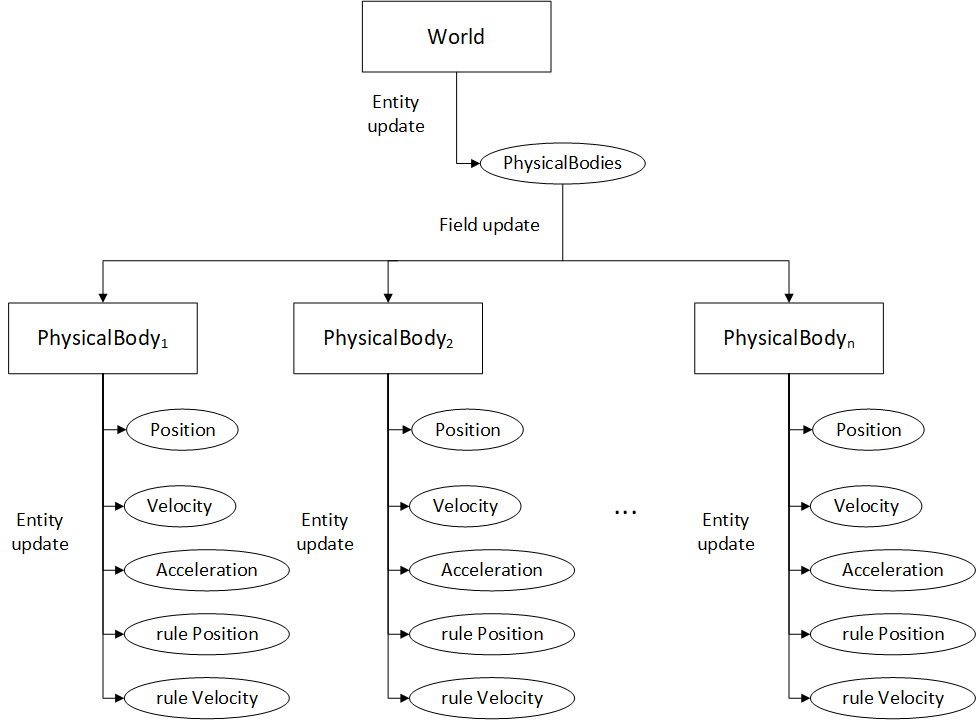
\includegraphics[width=\textwidth]{Figures/chapter_networking/update_traversal}
	\caption{Entity update for the simulation of physical bodies}
	\label{fig:ch_networking_simulation_update}
\end{figure}

\subsection{Update in Metacasanova}
\label{subsec:ch+networking_update_metacasanova}
The update mechanism described in Section \ref{subsec:ch_networking_casanova_update} can of course be integrated in the implementation of Casanova described in Chapter \ref{ch:languages}. In order to do so, we should dynamically look into the dictionary at each update, extract the field and perform an update according to the following cases:

\begin{itemize}[noitemsep]
	\item If the field is a list, then we must examine each element and choose for each one whether it needs to be updated or not. This is done by recursively applying these cases.
	\item If the field is a tuple, then we behave as above.
	\item If the field is an entity, then we must run an update on it.
	\item In all the other cases the field is not updated.
\end{itemize}

\noindent
The cases above are translated into four rules in Metacasanova. The first three will use pattern-matching to decide whether the examined field is a list, a tuple, or an entity. The fourth one is a default rule that simply returns the field as it is. Moreover, each entity should carry with it a list of rules that are updated as well, where all the get and set operations require dynamic lookups in the symbol table of the entity.

Repeating the traversal of the entity tree at each update at runtime is unnecessary since

\begin{itemize}[noitemsep]
	\item The structure of a Casanova entity cannot change at runtime. Its fields and field types will always remain the same.
	\item The fields affected by an entity rule and the rules of an entity do not change during the program execution.
\end{itemize}

\noindent
This means that, by exploiting modules and functors, we are able to specify the structure of the update at compile time and generate directly the function that performs the update at runtime, in the same fashion of what had been done for the record setter and getter. In the following sections we will describe extensively the implementation of the update using modules and functors in Metacasanova that generates at compile time the functions necessary to perform the update of a Casanova program. Note that we will refer to the implementation of records given in Section \ref{sec:ch_functors_record_implementation}.

\subsection{Updater Modules}
\label{subsec:ch_networking_updater_modules}
As explained above, Casanova needs to recursively update fields that are lists, tuples, or entity instances. At this purpose, we define a module that represents an \textit{updatable element} in the Casanova language. The module constructor takes as only argument the type of the element to update. This module contains a function \texttt{update} that is able to update a value of this particular type and uses an additional parameter \texttt{dt} that contains the time difference between the current and the previous update. The function returns the updated value of the element. It also contains an utility functor for the 
 
\begin{lstlisting}
Module "ElementUpdater" => (elementType : *) : ElementUpdater {
	Functor "GetType" : *
	Func "update" -> elementType -> float : elementType
}
\end{lstlisting}

\noindent
The updater for a field is a module constructed by providing the record of the fields, its name as a string, and contains: (\textit{i}) an utility functor that returns the record used in the field updater, and (\textit{ii}) an update function that takes as input an instance of the record, \texttt{dt}, and returns the updated value of the field. We also define an external utility functor \texttt{GetFieldType} that can retrieve the type of a record field given the record it belongs to and its name. The rule for the functor calls the field getter and its \texttt{GetType} functor to retrieve the type of the name. This functor is used by the module constructor to correctly generate the return type of the \texttt{update} function.

\begin{lstlisting}
Functor "GetFieldType" => Record => string : *

GetField r name => getter
getter.GetType => type
---------------------------
GetFieldType r name => type

Module "FieldUpdater" => (r : Record) => (name : string) : FieldUpdater {
  Functor "GetRecord" : Record
  Func "update" -> r.RecordType -> float : (GetFieldType r name)
}
\end{lstlisting}

\noindent
Finally, the updater for a record is a module constructed by providing the record itself and contains: (\textit{i}) an utility functor that returns the type of the record, and (\textit{ii}) a function \texttt{update} that takes the instance of the record, \texttt{dt}, and returns an updated instance of the record.

\begin{lstlisting}
Module "RecordUpdater" => (r : Record) : RecordUpdater {
  Functor "RecordType" : *
  Func "update" -> r.RecordType -> float : r.RecordType
}
\end{lstlisting}

\subsection{Updatable elements}
\label{subsec:ch_networking_updatable_elements}
As explained above, the elements for which the update is needed can be lists, tuples, or entity instances. For this reason we have to create separately three different instances of the module \texttt{ElementUpdater} each one dedicated to updating one of those updatable elements. The first updatable element that we consider is an \textit{entity instance}. The module to update such updatable element uses a \texttt{RecordUpdater} to define how to entity instance should be updated. Indeed updating a field containing an entity instance requires to apply the specific updater for that entity, which in turn returns the updated instance of the entity itself. Thus the declaration for the functor that constructs the proper instance of the module for the entity updater is the following:

\begin{lstlisting}
Functor "UpdateEntity" => RecordUpdater : ElementUpdater
\end{lstlisting}

\noindent
The rule for this functor extract in its premise the type of the record by calling the utility functor \texttt{RecordType} in the record updater passed as parameter to the constructor of the module. The \texttt{update} function uses the record updater to recursively update the entity instance in its premise and then returns the result of this update.

\begin{lstlisting}
recordUpdater.RecordType => recordType
--------------------------
UpdateEntity recordUpdater => ElementUpdater recordType {

	----------------------
	GetType => recordType
 
  recordUpdater.update entity dt -> entity'
  ------------------------------
  update entity dt -> entity'
}
\end{lstlisting}

\noindent
The second updatable element is the list. An updater for a list must take the updater for its elements. Since a list contains elements of the same type, only one updater is required to instantiate its updater module. The functor \texttt{UpdateList} used to generate this module takes one argument which is an \texttt{ElementUpdater}. This is done because the elements of a list could be themselves other lists, entities, or tuples, so we must be able to use their updaters as arguments for this function. The declaration for this functor is thus:

\begin{lstlisting}
Functor "UpdateList" => ElementUpdater : ElementUpdater
\end{lstlisting}

\noindent
The rule for \texttt{UpdateList} extracts in its premise the type of the elements of the list by calling the functor \texttt{GetType} in the element updater provided as input. It then instantiates an \texttt{ElementUpdater} with the type \texttt{List} using as argument for the generic type the type of the element extracted in its premise. The \texttt{update} function for the list is recursive: its base case is the empty list, for which it simply returns an empty list. For a non-empty list the rule for this function uses the element updater in its premise to update the head of the list and then recursively calls the \texttt{update} of the list on the tail to updater the remaining part.

\begin{lstlisting}
updater.GetType => elementType
---------------------------------
UpdateList updater => ElementUpdater List[elementType] {

  -----------------
  GetType => List[elementType]

  --------------------
  update nil dt -> nil

  updater.update x dt -> x'
  update xs dt -> xs'
  -------------------
  update (x :: xs) dt -> (x' :: xs')
}
\end{lstlisting}

\noindent
The updater for tuples is built by defining a functor that takes as input two element updaters, one for the current element of the tuple, and one for the second one. Note that it is possible to recursively provide a tuple updater as a second updater to support the update of tuples containing more than two elements. For example, the updater for \texttt{Tuple[PhysicalBody,Tuple[PhysicalBody,\\PhysicalBody]]} would require to pass an entity updater and recursively a tuple updater. The declaration of this fuctor is thus:

\begin{lstlisting}
Functor "UpdateTuple" => ElementUpdater => ElementUpdater : ElementUpdater
\end{lstlisting}

\noindent
The rule for \texttt{UpdateTuple} uses in its premises \texttt{GetType} from the first updater and the second updater to obtain the types of the first and second element of the tuple. It then instantiates \texttt{ElementUpdater} with the tuple type called with the type of the first and second element as arguments for the generics. The \texttt{update} function runs the \texttt{update} of the first updater on the first element of the tuple and the second updater on the second element.

\begin{lstlisting}
updater.GetType => firstType
nextUpdater.GetType => nextType
---------------------------------------------
UpdateTuple updater nextUpdater => ElementUpdater Tuple[firstType,nextType] {

  -------------------
  GetType => Tuple[firstType,nextType]

  updater.update x dt -> x'
  nextUpdater.update x' dt -> xs'
  ----------------------
  update (x,xs) dt -> (x',xs')
}
\end{lstlisting}

Finally, we need a \texttt{ZeroUpdate} that is required for fields whose values do not change with respect to time, namely all those that do not fall in the three categories above. The functor \texttt{ZeroUpdate} takes as input any type and builds an \texttt{ElementUpdater} with that type. The rule for \texttt{update} simply returns the value of the field as it is.

\begin{lstlisting}
Functor "ZeroUpdate" => * : ElementUpdater

-----------------------
ZeroUpdate type => ElementUpdater type {

  ----------------
  GetType => type

  ----------------
  update v dt -> v
}
\end{lstlisting}

\subsection{Updatable Fields and Records}